\section{Topic Modeling Evaluation}

    \graphicspath{{Chapter4/Figures}{Chapter4/Figures}}

This section presents the evaluation of different models used for tweet labeling. Both unsupervised and supervised approaches were used to evaluate the performance of the models. The evaluation aimed at finding the best-performing model to label tweets accurately. The models included traditional methods (LDA, GSDMM, and NMF) and neural models like BERTopic.

The unsupervised evaluation (\ref{sec:unsupervised}) assessed the traditional metrics used in this context, such as coherence and diversity scores. The results showed that BERTopic performed better than traditional methods, especially when using all-MiniLM-L6-v2 (BERT) \footnote{\href{https://huggingface.co/sentence-transformers/all-MiniLM-L6-v2}{huggingface.co/sentence-transformers/all-MiniLM-L6-v2}}
, text-embedding-ada-002 (OpenAI) \footnote{\href{https://platform.openai.com/docs/models/embeddings}{platform.openai.com/docs/models/embeddings}},
and tweet\_classification \footnote{\href{https://huggingface.co/louisbetsch/tweetclassification-bf-model}{huggingface.co/louisbetsch/tweetclassification-bf-model}} embeddings. 


The supervised evaluation consisted in building a custom-labeled dataset from scratch, and then in looking at the accuracy of the models. The results showed that BERT and OpenAI were the best-performing models. The section culminates with a summary of the results and a description of the representation used for labeling the tweets.

The models used are both traditional (LDA, GSDMM, NMF), as a reference of the ground truth, and neural, because they seem to be the most accurate; in particular, BERTopic will be evaluated with several embedding methods.  BERtopic was chosen over Top2Vec both because they are very similar, and because the Python library is more comprehensive and allows for more flexibility.

Evaluating a topic modeling algorithm is challenging due to the lack of objectivity in identifying a topic. In this work, the models were evaluated in two ways: firstly, by employing a widely used unsupervised approach: metrics like coherence and diversity. Then, to validate the results, a supervised evaluation was also carried out by using different datasets built ad hoc for this setting.

\subsection{Unsupervised}
\label{sec:unsupervised}
To compare the different models, a library suggested by the creator of BERtopic called OCTIS \cite{DBLP:conf/clic-it/TerragniF21} \cite{terragni2020octis} was used; this allowed the creation of an experiment to measure the different metrics presented in chapter \ref{Ch:related}: coherence and diversity.




\paragraph{Dataset}
In this case, the dataset is composed of 1669 preprocessed tweets related to climate change with the hashtag \textit{\#cop22}, all in english; the preprocessing phase involved removing retweets, links, punctuation, and the most common hashtags (\#cop22, \#climatechange \#p2).  We choose this dataset, which is not the one used in the final analysis because the domain is the same, and the goal analogous, since we have to detect subtopics of a main topic which is climate change. For this reason we can generalize the result to the tweets of the other COPs.

\paragraph{Methods}

The models used in this evaluation were LDA, NMF, and BERTopic. In the BERtopic case, several embeddings have been tested (  all-MiniLM-L6-v2, text-embedding-ada-002, climatebert \cite{webersinke_climatebert_2022}, tweet\_classification, USE \cite{cer_use_2018}).

Each model has been fitted several times changing the parameters:
\begin{itemize}
    \item  \textbf{number of topics} from 10 to 50 with a step of 5 
    \item \textbf{min topic size}: 5 and 15  tweets\footnote{only for bertopic}
\end{itemize}


Each unique combination of parameters has been fit three different times; then, we took the mean value of the three computations.

\paragraph{Results}
The results show that BERtopic performs way better in these tests than the traditional methods. In comparison, the best Bertopic embeddings are mini, OpenAi, and tweet classification.
The experiment demonstrates how the $min\_topic\_size$ value of 5 is too small, thus the results will be gathered considering a value of 15.

Fig \ref{figure:unsupervised_results} shows the value of all the metrics with a different number of topics for the traditional methods and the best-performing neural one (OpenAI)

\begin{figure}[h]
    \centering % figure is centered on the page
        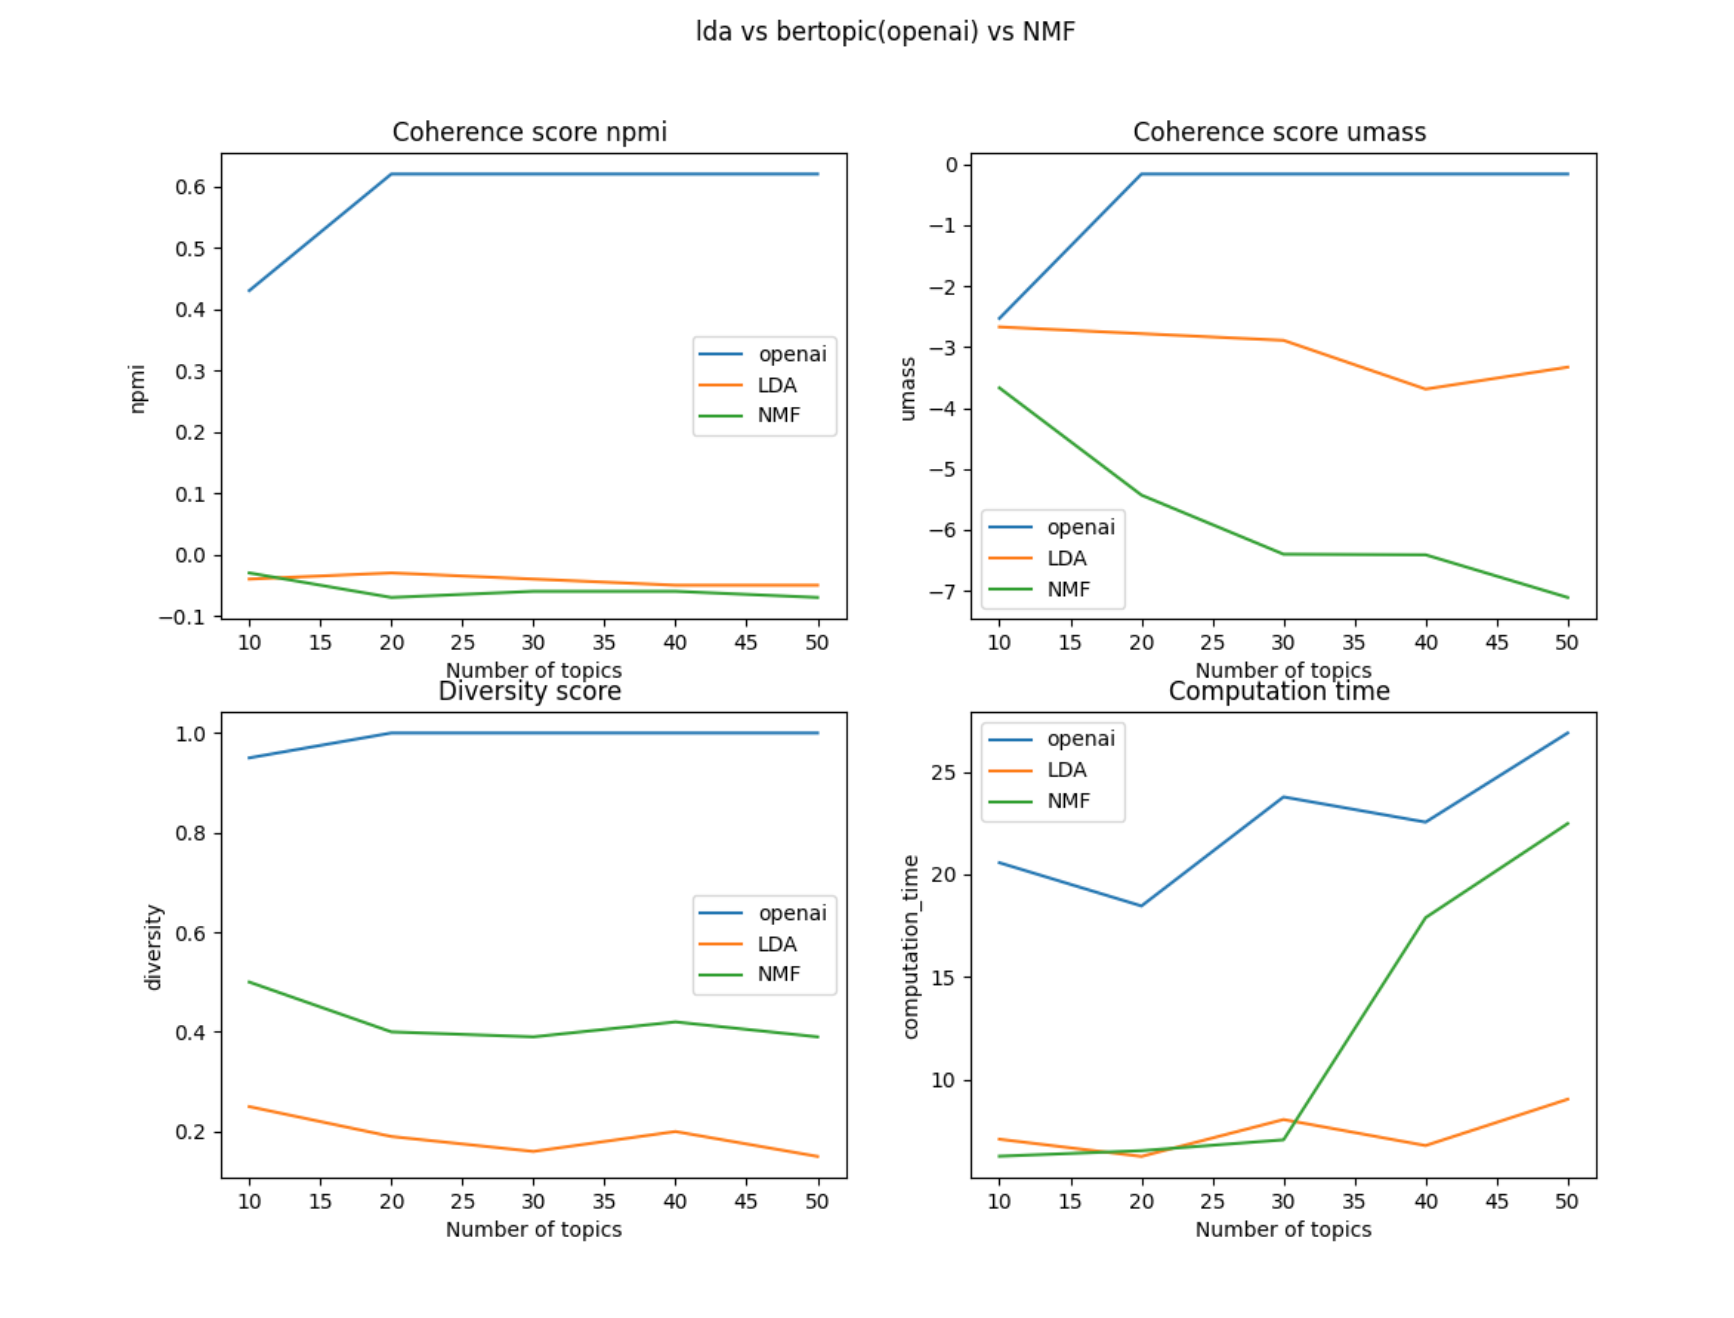
\includegraphics[width=0.99\linewidth]{Chapter4/figures/topic_unsupervised.png} 
    \caption{coherence and diversity for LDA, BERTopic, and NMF
    }
    \label{figure:unsupervised_results} 
\end{figure}


However, Hoyle et al. \cite{hoyle_is_2021} explained how these metrics are not very meaningful for the evaluation of these models due to the lack of validation for neural models, therefore  these results should be taken with a grain of salt.

From this evaluation, it can be concluded that BERTopic’s topic size is better bigger than smaller, especially if many documents are available. Topics of Bertopic are way more diverse than the ones of LDA and NMF and, within the topics, the most relevant words are more semantically related.


\begin{table}[]
\centering
\begin{tabular}{|llll|}
\hline
\textbf{model}                              & \textbf{npmi} & \textbf{umass} & \textbf{diversity} \\ \hline
\multicolumn{1}{|l|}{tweet\_classification} & 0.62          & -0.16          & 1                  \\
\multicolumn{1}{|l|}{openai}                & 0.58          & -0.63          & 0.99               \\
\multicolumn{1}{|l|}{climatebert}           & 0.20          & -2.28          & 0.83               \\
\multicolumn{1}{|l|}{U.S.E}                 & 0.20          & -4.35          & 0.89               \\
\multicolumn{1}{|l|}{BERT}                  & 0.20          & -5.46          & 0.97               \\
\multicolumn{1}{|l|}{LDA}                   & -0.04         & -3.07          & 0.19               \\
\multicolumn{1}{|l|}{NMF}                   & -0.06         & -5.80          & 0.42               \\ \hline
\end{tabular}
\caption{all the models tested in the unsupervised evaluation}
\label{tab:unsupervised_recap}
\end{table}


\subsection{Supervised}
Considering the result of the unsupervised evaluation, another method should be used to validate what was found. In this case, two ad-hoc datasets were created to see how the models perform in a real-case scenario.
\paragraph{Dataset}

The first step for the supervised phase was the data collection. In this case,  specific datasets were packed to test the chosen models. The datasets were selected based on the trending topic on Twitter at the time (March 2023).
The first dataset is simpler and contains very different topics, it follows that it should be effortless enough to cluster the documents. In contrast, the second dataset is trickier because it includes only politics-related tweets, including some which overlap with more hashtags related to US politics.


\begin{itemize}
    \item \textbf{simple}: 1093 labeled tweets of 5 different topics identified by a hashtag \footnote{\#Bitcoin, \#stormydaniels, \#UkraineRussianWar, \#SaudiArabianGP, \#climatechange}
    \item \textbf{politics}: 1492 labeled tweets of 7 politics-related hashtags \footnote{\#IndictArrestAndConvictTrump, \#kabul, \#BidenHarris2024, \#KamalaHarris, \#taiwan, \#belarus,  \# stormydaniels}
\end{itemize}


For both datasets, we used two different versions: with and without hashtags. The reason beheind this was to avoid the risk of the model to cluster based on the hashtags.

The tweets have been extracted using \href{https://twarc-project.readthedocs.io/en/latest/twarc2_en_us/}{twarc2}, getting only English tweets and excluding retweets. Only the trending topic at that time (March 2023) was used because Twitter API did not allow access to data before 48h.

\paragraph{Metrics}
In order to evaluate the topics, it was necessary to define some accuracy metrics, which is not a straightforward task because, by using BERTopic, there is no set number of topics apriori, but it has to figure it out by itself.
After running the model, both the known topic (the hashtag) and the inferred one (a number) are established, making it possible to create a confusion matrix between the two sets. To map the inferred topic to the known one, the inferred topic with the highest value was considered. In the case at hand, the error can be detected  by combining this value with another metric: min\_topic\_size.

The metrics defined are the following:

\begin{itemize}
    \item \textbf{Accuracy}: for each known topic, take the biggest inferred topic of the same row of the confusion matrix and divide by the number of tweets in that topic, fig \ref{figure:supervised heatmap1} can be taken as reference.
    \item \textbf{Accuracy no outliers}: in the Bertopic case, the label -1 refers to outliers. Therefore, to achieve it, compute the same as for accuracy but without counting the outliers.
    \item \textbf{Min\_topic\_share}: same as for accuracy but in the opposite direction, after having computed it for all of inferred topics, the minimum is considered. This is helpful to detect when the accuracy is considering the wrong topic, which could happen when the inferred topic size is less than the actual topic one (so one inferred topic contains tweets from multiple topics, and then this number is low)
\end{itemize}


\paragraph{Parameters}

$max\_df$ is used to remove the terms that appear too frequently; a value of 0.95 means remove the terms that appeared in more than 95\% of documents, while 
$min\_df$ is the opposite; in this case, with the value being an integer, the parameter refers to the minimum number of documents a term should be in to be considered.

$Alpha$ is a parameter that influences the number of clusters that will be created; low alpha results in many clusters with single words, while high alphas results in fewer clusters with more words.
For these 3 the default settings were used.


$ngram\_range$  defines the number of consecutive words to be considered: for example, a value of (1,2) tells the method to consider single words and bigrams (two consecutive words), but including threegrams was too computationally expensive.

 A $min\_topic\_size$ of 50 was made because 200 tweet for each hashtag were inspected and, considering that some of them will be classified as outliers, a size of 50 was a safe trade-off in order not to risk that a topic nor the size were too small since, from unsupervised evaluations, it was  concluded that the bigger the size, the better.

\begin{verbatim}
BERTopic: (nr_topics = 'auto', min_topic_size = 50)

NMF: (max_df = 0.95, min_df = 3, ngram_range = (1,2))

GSDMM: (alpha = 0.1, min_df = 0.1, n_iters = 30)
\end{verbatim}


\paragraph{Simple Dataset Results}
 At first, the evaluation was on the simple dataset with hashtags. As Fig 4.2 shows, base ( all-MiniLM-L6-v2) and OpenAi obtained almost a perfect score for each topic. At the same time, climatebert seems to have a great accuracy but a low mean topic share, this is a signal that something is wrong and the heatmap should be inspected.

\begin{figure}[h]
    \centering % figure is centered on the page
        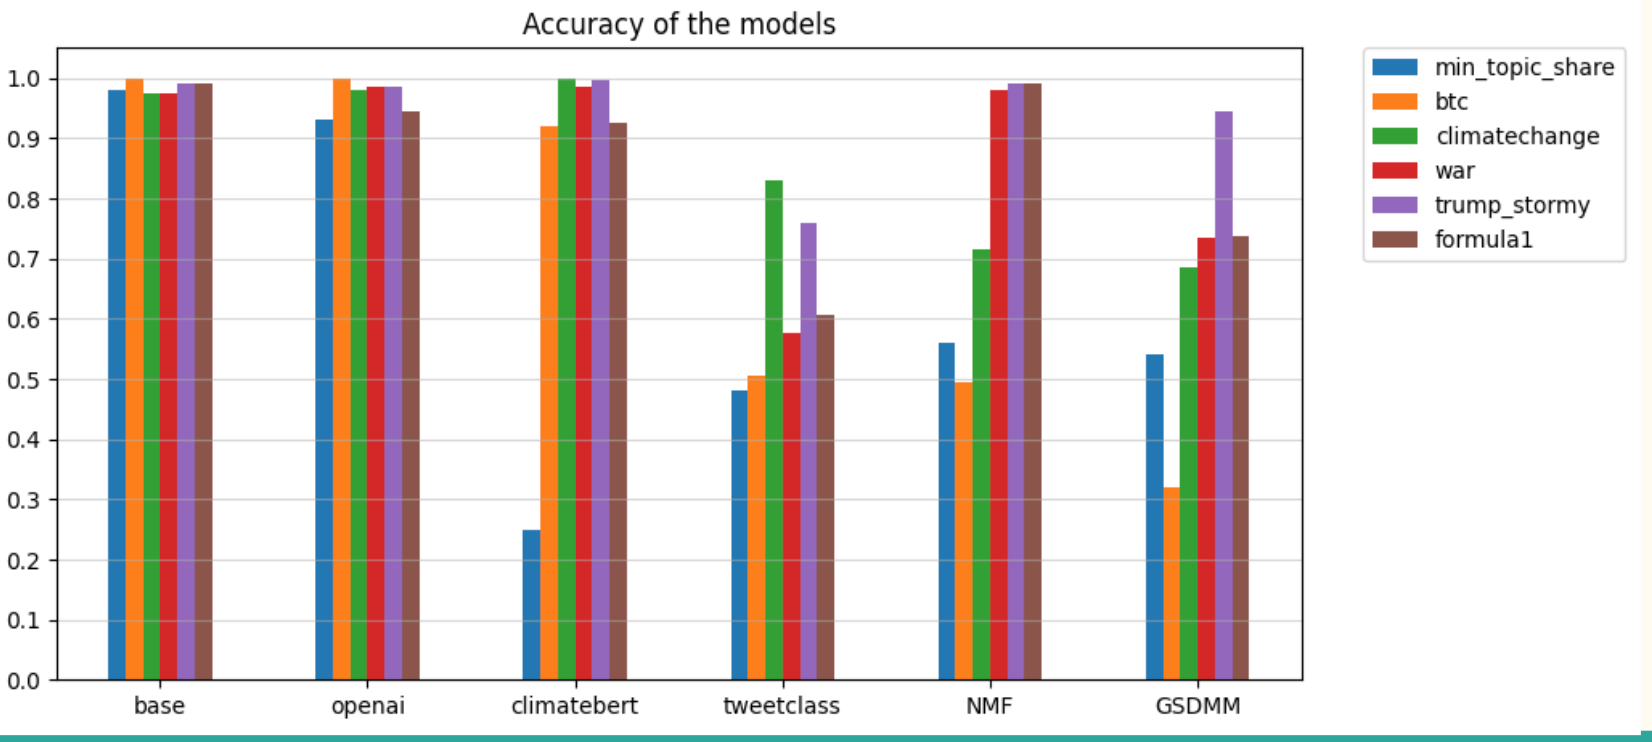
\includegraphics[width=0.99\linewidth]{Chapter4/figures/topic_supervised_bar.png} 
    \caption{All models accuracy simple  with hashtags
    }
    \label{figure:supervised bar} % assign a unique label to each figure
\end{figure}

In fact, it is clear from  \ref{figure:sup_heatmap1_simple_hash} that even though the accuracy is very good, climatebert has some difficulties in dividing the topics, putting almost all the tweets in the same inferred topic. While the first two are performing very well as expected, the same is not true for the others.  Climatebert puts almost all the tweets in topic 0, thus being able only to find the formula1 tweets and not the climatechange one, as it is designed to do. That’s the reason why the decision was to remove the models that were not performing well in the simplest case, with the exception of NMF to use as ground truth.


\begin{figure}[h]
    \centering % figure is centered on the page
        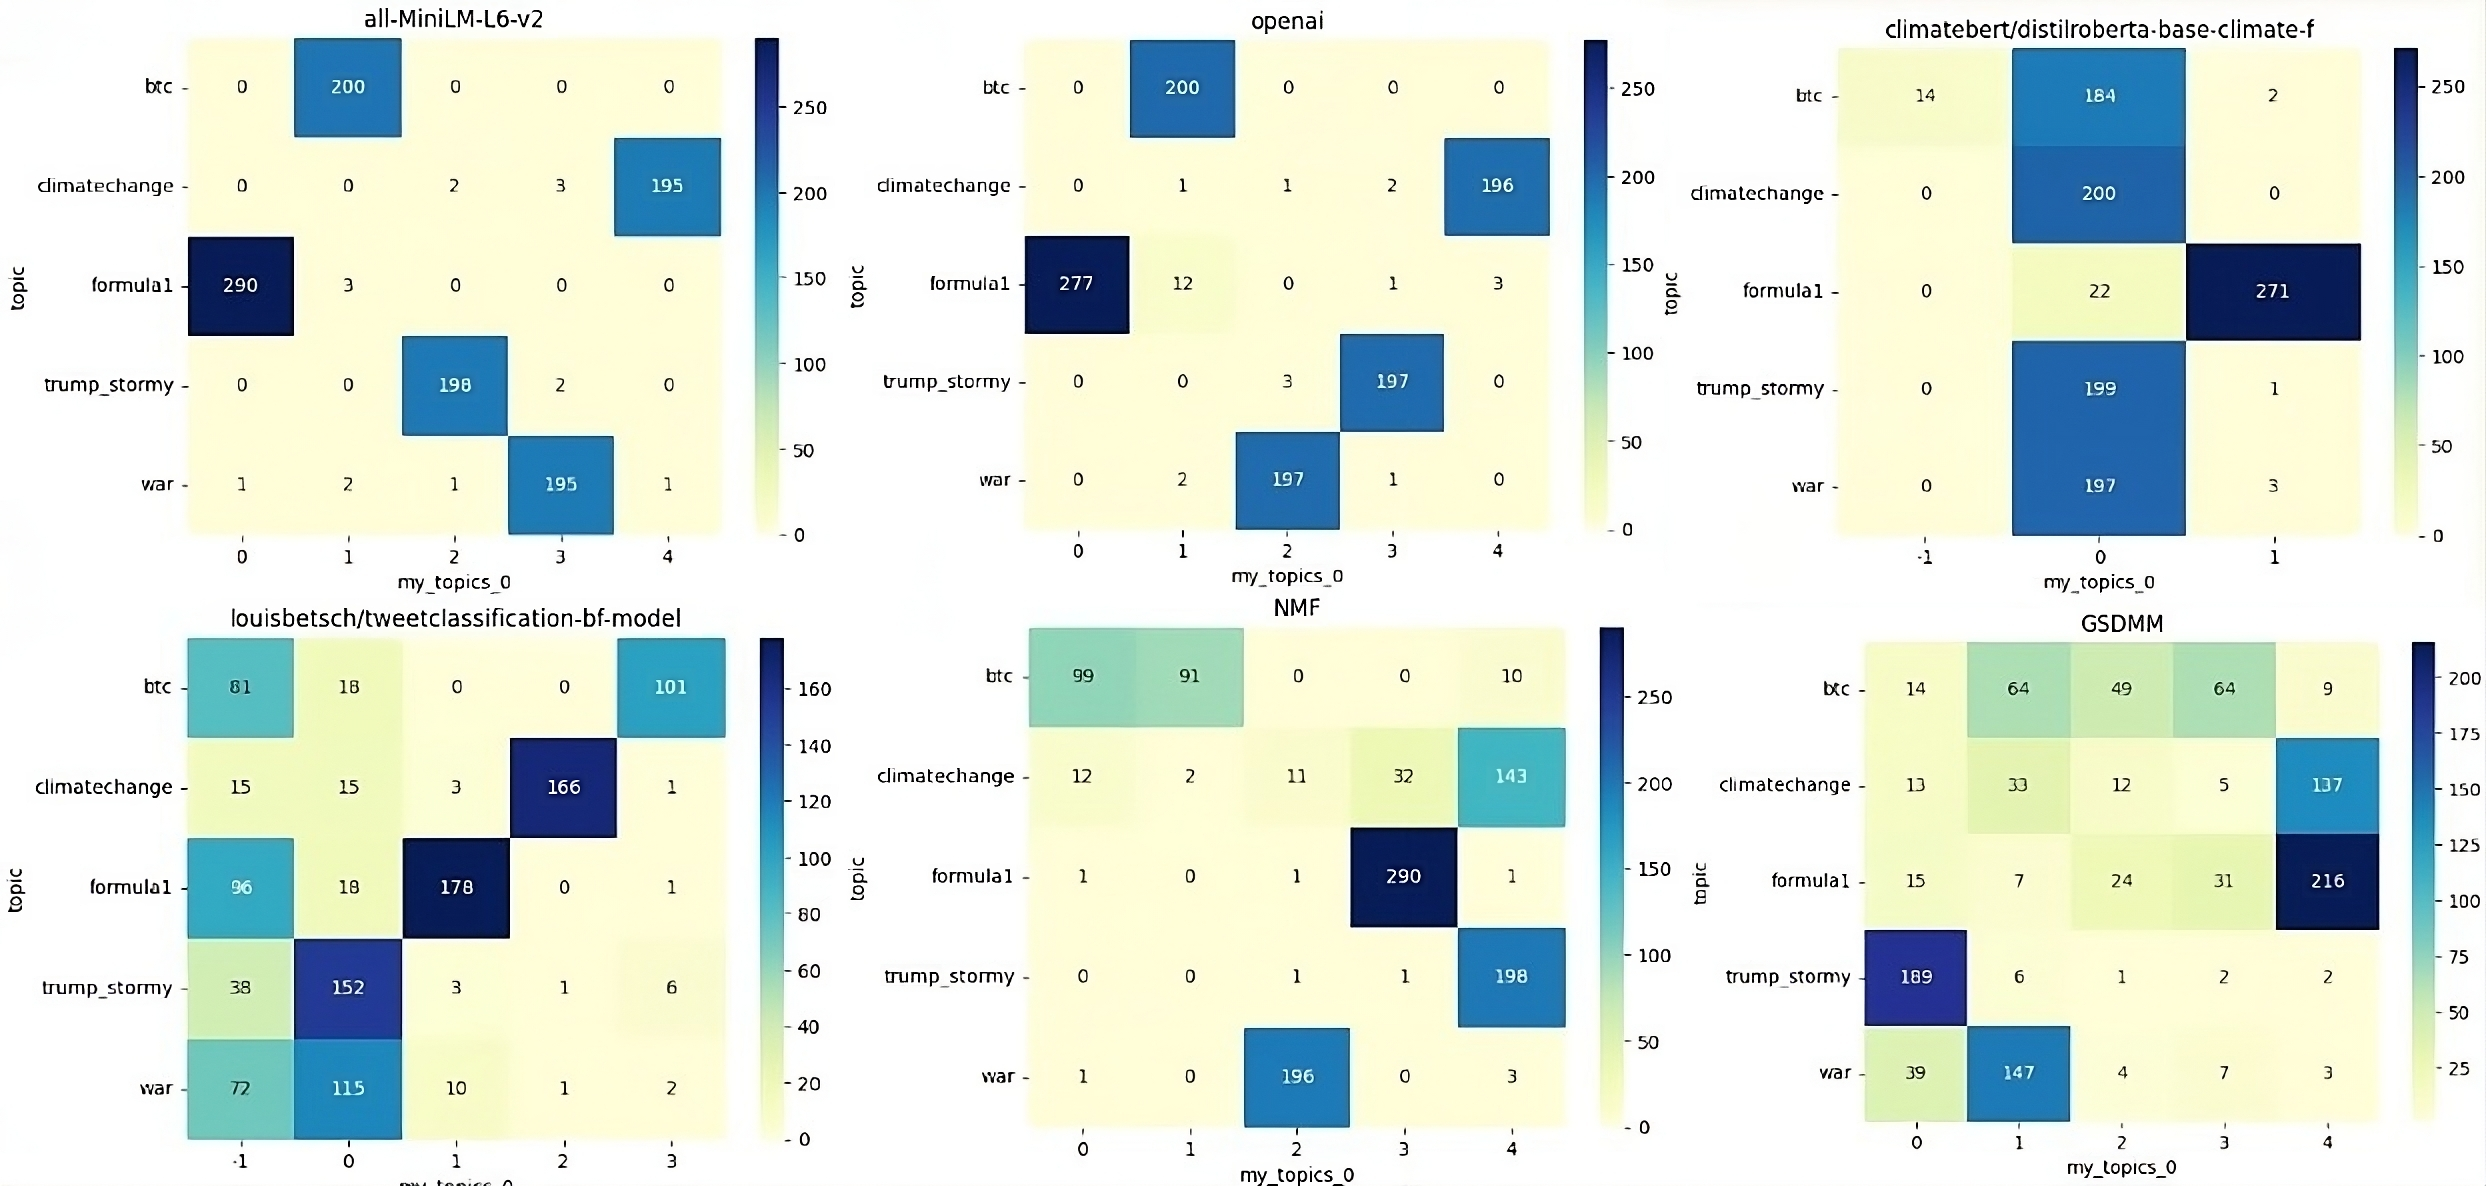
\includegraphics[width=0.99\linewidth]{Chapter4/figures/heatmaps_eval.jpeg} 
    \caption{Heatmap comparison of the different model with the simple dataset with hashtags
    }
    \label{figure:sup_heatmap1_simple_hash} % assign a unique label to each figure
\end{figure}

Fig \ref{figure:supervised heatmap1} shows how BERT and OpenAI performed in the simple dataset but without the hashtags and, in particular, how BERT tends to find more outliers than OpenAI. Overall, both get a good performance.


\begin{figure}[h]
    \centering % figure is centered on the page
        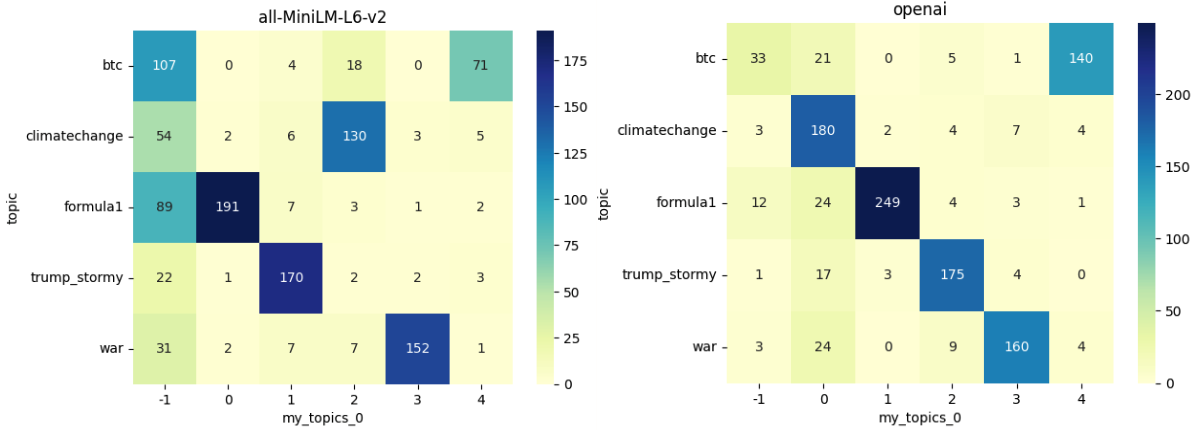
\includegraphics[width=0.99\linewidth]{Chapter4/figures/bert_vs_openai_heatmap.png} 
    \caption{Heatmap comparison of mini and OpenAi of the simple dataset without hashtags}
    \label{figure:supervised heatmap1} % assign a unique label to each figure
\end{figure}

An interesting feature of Bertopic is the ability to visualize the different topics in 2-dimensional space; Fig \ref{fig:openai docs} shows the document distribution of OpenAi after reducing the dimensionality of the embeddings .

\begin{figure}
    \centering
    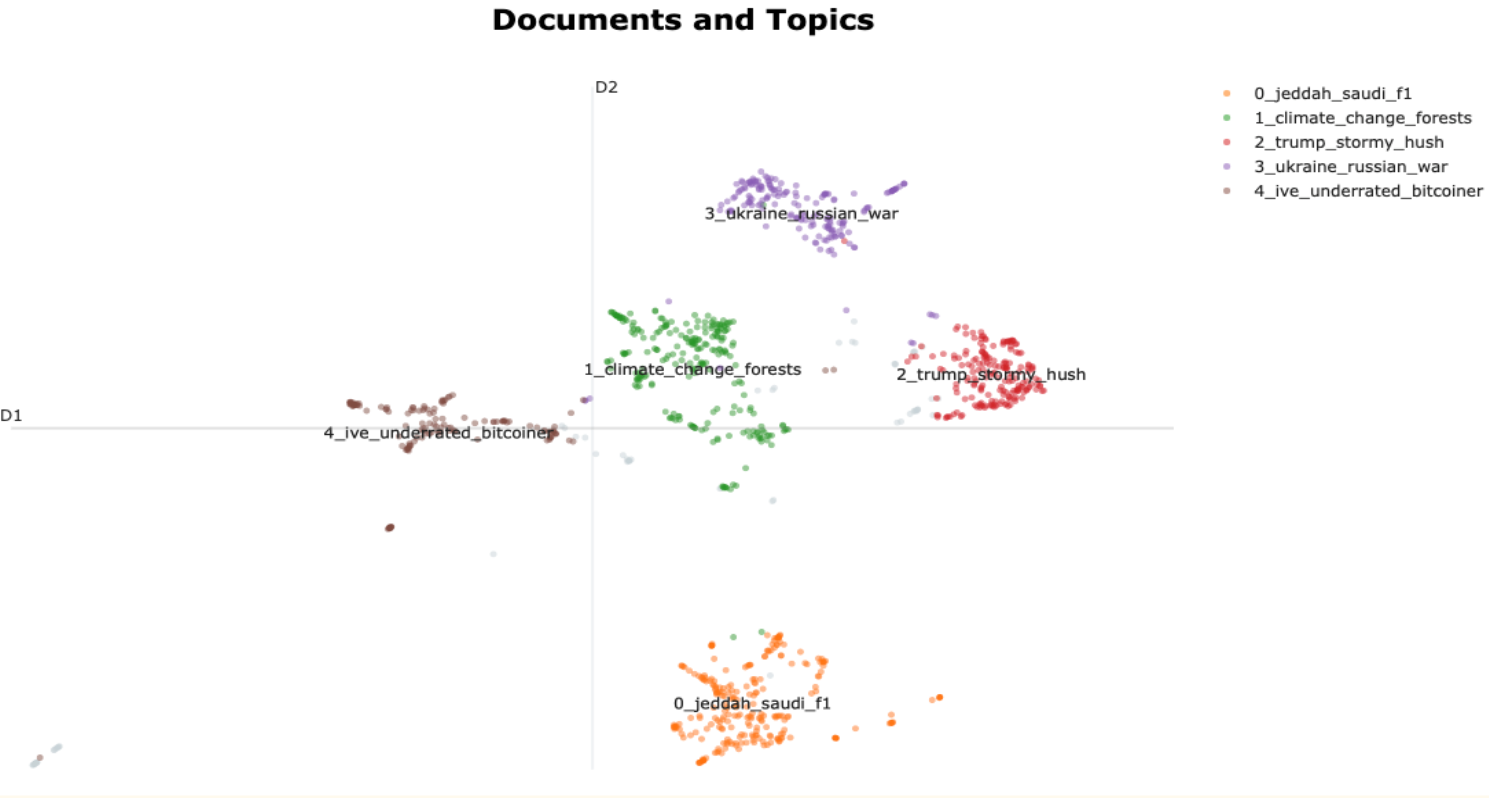
\includegraphics[width=1\linewidth]{Chapter4/figures/openai_doc_viz.png}
    \caption{docs representation of simple dataset for openai}
    \label{fig:openai docs}
\end{figure}


\paragraph{Politics dataset results}

The politics dataset is clearly more difficult to evaluate, but with the hashtags, it is still doing a good job. Fig \ref{fig:openai_heat_docs_politics_hash} \ref{fig:bert politics with hashtags} shows heatmap and topic distribution for the politics dataset with hashtags.

 Both BERT and OpenAi are creating two topics from the Taiwan case. OpenAi merges two topics, which is coherent with the fact that the two hashtags related to Trump are also related to the same event( \#IndictArrestAndConvictTrump and \#stormydaniels). 

\begin{figure}
    \centering
    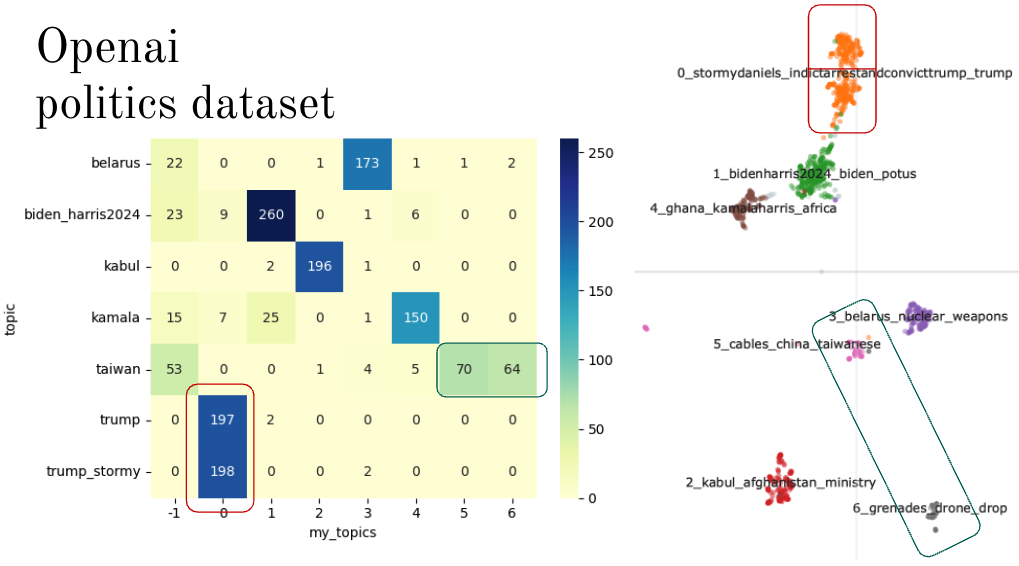
\includegraphics[width=1\linewidth]{Chapter4/figures/heatmaps_documents_openai.png}
    \caption{Heatmap and documents representation of the politics dataset with hashtags evaluated with openai}
    \label{fig:openai_heat_docs_politics_hash}
\end{figure}

To validate the results, the algorithm was run 100 times and, most of the time, for BERT the min topic share was 0.9, which means it got the correct number of topics and classified them in a good way.

\begin{figure}
    \centering
    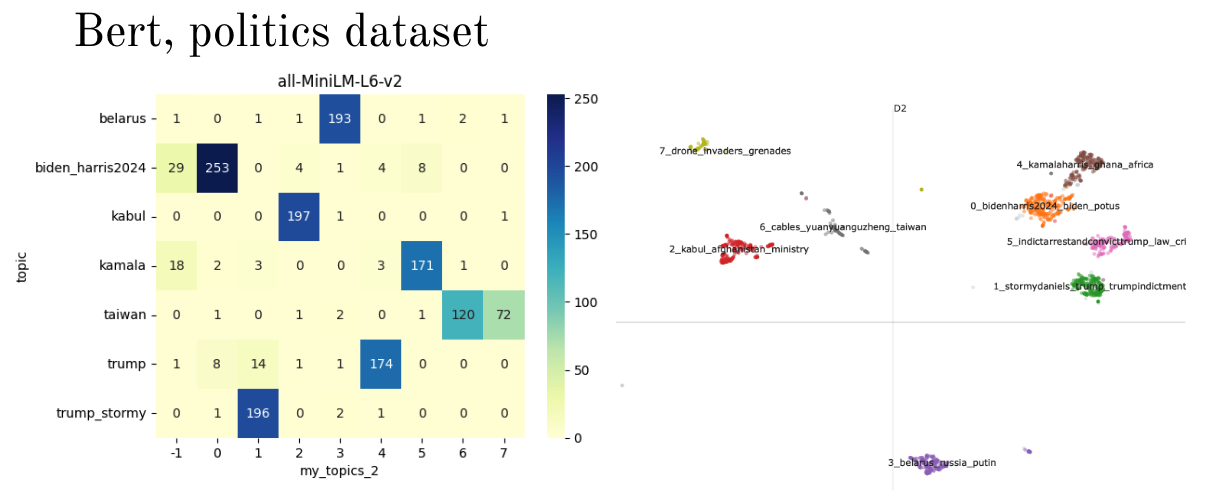
\includegraphics[width=1\linewidth]{Chapter4/figures/heatmaps_docs_bert.png}
    \caption{bert heatmap and document viz politics with hashtags}
    \label{fig:bert politics with hashtags}
\end{figure}

In the case without hashtags, OpenAi and BERT put in a single cluster all the tweets related to American politics, both also understanding that Kamala's tweets were about something else.


\paragraph{Topic representation}
The last step is giving a meaningful label to the clusters created, so that it can be seen if the openai API works well; in particular, the model named \textit{gpt-3.5-turbo} was used, which worked surprisingly well; table \ref{tab:supervised_labels} contains the label generated for both simple and political datasets.

Fig \ref{fig:openai_heat_docs_politics_hash} as reference. Note that the discussion under the \#taiwan hashtag is divided into two different topics, as depicted in the document representation.

The prompt used is: \textit{you are a tweet labeler, you are given representative words from a topic and three representative tweets, give more weight to the words, given all this information give a short label for the topic (max 10 words), starts all with topic:}


\begin{table}
\begin{tabular}{ll}
\hline
\textbf{simple dataset}            & \textbf{label}                                             \\ \hline
\#Bitcoin                          & Cryptocurrencies                                            \\
\#stormydaniels                    & Trump's hush money payment to Stormy Daniels.              \\
\#UkraineRussianWar                & Ukraine-Russia conflict                                    \\
\#SaudiArabianGP                   & F1 Saudi Arabian Grand Prix 2023                           \\
\#climatechange                    & Forests and Climate Change                                 \\ \hline
\textbf{politics dataset (openai)} &                                                            \\ \hline
\#IndictArrestAndConvictTrump      & Stormy Daniels controversy                                 \\
\#stormydaniels                    & Stormy Daniels controversy                                 \\
\#kabul                            & Suicide bombing near foreign ministry in Kabul             \\
\#BidenHarris2024                  & Politics and Leaders                                       \\
\#KamalaHarris                     & Kamala Harris official visit to Ghana and Africa           \\
\#taiwan                           & Tensions between China and Taiwan over undersea cables cut \\
\#taiwan                           & use of small drones for warfare'                           \\ \hline
\end{tabular}
\caption{labels generated using GPT API both for simple and political dataset
}
\label{tab:supervised_labels}
\end{table}

\paragraph{Conclusion}
Tab \ref{tab:unsupervised_recap} shows the result of unsupervised evaluation, while Tab \ref{tab:supervised recap } shows the supervised. Through the supervised evaluation, it is demonstrated  how the results of the unsupervised one were not completely true; this helped to discard some models and confirm the hypothesis that the neural model with Bert Embedder and Openai was the best performing model. There is still a significant difference between the two: Bert is open source and can be run locally, while Openai is not free and can only be used through API.



\begin{table}[]
\centering
\begin{tabular}{|l|ll|}
\hline
model  & accuracy & topic share \\ \hline
BERT   & 0.84     & 0.86        \\
OpenAI & 0.83     & 0.85        \\
NMF    & 0.78     & 0.69        \\ \hline
\end{tabular}
\caption{recap of supervised evaluation}
\label{tab:supervised recap }
\end{table}


